\documentclass{beamer}
\usetheme{Madrid}
\usecolortheme{whale}

\usepackage[utf8]{inputenc}
\usepackage{bookmark}
\usepackage{graphicx}
\usepackage{tikz}
\usetikzlibrary{arrows,shapes,positioning,shadows,calc}
\usepackage{colortbl}
\usepackage{xcolor}

\title{PI Protocol: Fullstack Privacy}
\subtitle{Logic Chaining \& Feature Implementation}
\author{Deep Dive Overview}
\date{March 2026}
\setbeamertemplate{footline}{} % Hide slide numbers

\begin{document}

\frame{\titlepage}

\begin{frame}{The Logic Chain: Data Journey}
    \begin{columns}
        \begin{column}{0.45\textwidth}
            How data moves safely:
            \begin{itemize}
                \item \textbf{Selection}: Java layer selects files/keywords.
                \item \textbf{Processing}: NDK invokes C++ PI Engine.
                \item \textbf{Tokenization}: FAST scheme generates 200k tokens.
                \item \textbf{Batched Sync}: Tokens sent in chunks of 5,000.
            \end{itemize}
        \end{column}
        \begin{column}{0.55\textwidth}
            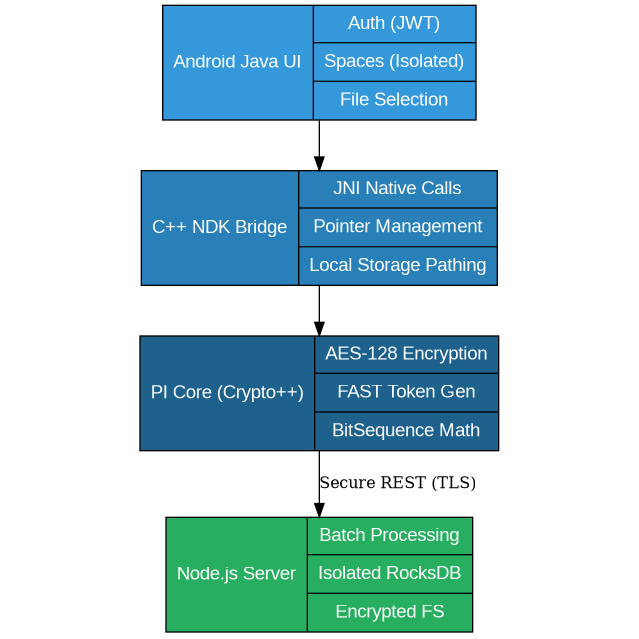
\includegraphics[width=\textwidth]{logic_chain_prog.png}
        \end{column}
    \end{columns}
\end{frame}

\section{Core Implementation Features}
\begin{frame}{Isolated Secure Spaces}
    \begin{columns}
        \begin{column}{0.6\textwidth}
            \textbf{Zero-Trust Isolation}:
            \begin{itemize}
                \item \textbf{Physical Separation}: Every space has a unique RocksDB + FS folder.
                \item \textbf{Unique Keys}: Private keys generated per-space; never leave the phone.
                \item \textbf{Session Security}: JWT authentication protects all space interactions.
            \end{itemize}
        \end{column}
        \begin{column}{0.4\textwidth}
            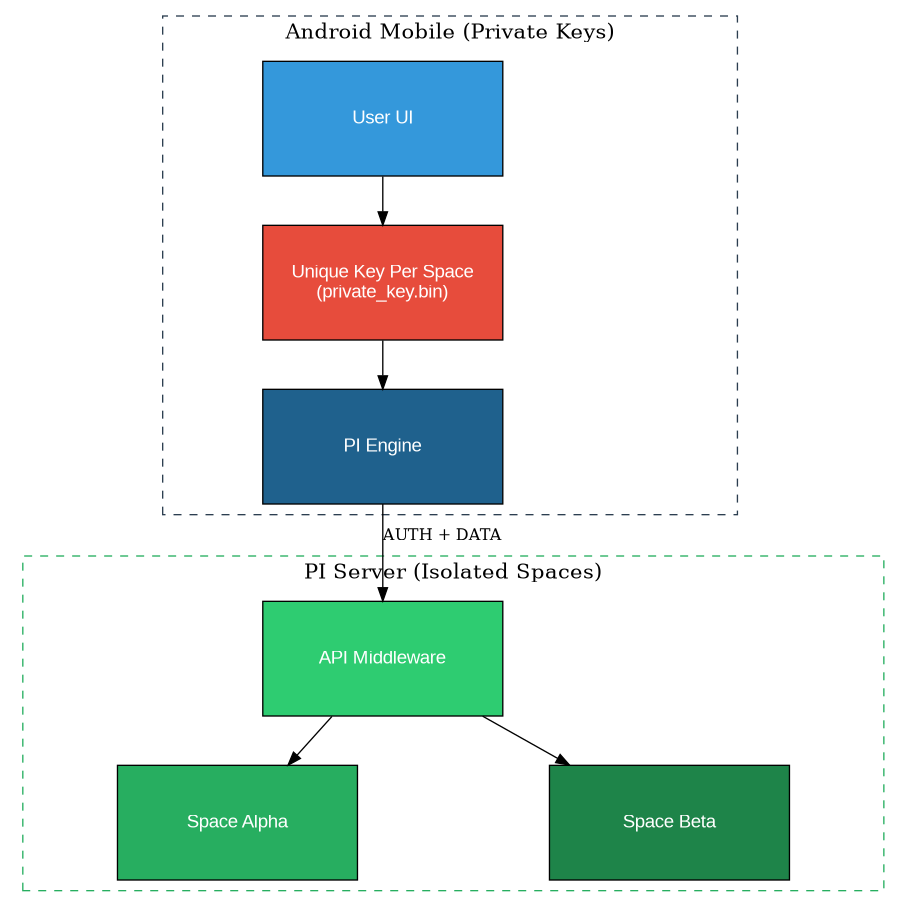
\includegraphics[width=\textwidth]{arch_prog.png}
        \end{column}
    \end{columns}
\end{frame}

\begin{frame}{Advanced Update \& Metadata}
    \begin{itemize}
        \item \textbf{Extension Preservation}: Encrypts \texttt{doc.pdf} to \texttt{ID0.pdf}. The server knows the extension (so storage works) but not the content.
        \item \textbf{Payload Batching}: The App prevents Out-Of-Memory (OOM) network crashes by chunking uploads into exactly 5,000-token arrays and 5-file bundles per HTTP POST.
        \item \textbf{Local State Management}: The phone tracks indexing state locally in a mini-RocksDB to prevent token collision.
    \end{itemize}
    \begin{center}
        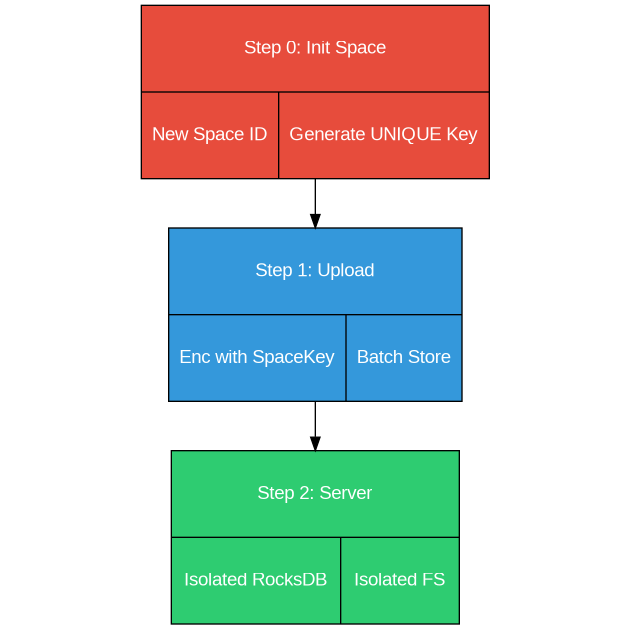
\includegraphics[height=0.4\textheight]{scheme_prog.png}
    \end{center}
\end{frame}

\begin{frame}{Private Search Strategy}
    \begin{columns}
        \begin{column}{0.5\textwidth}
            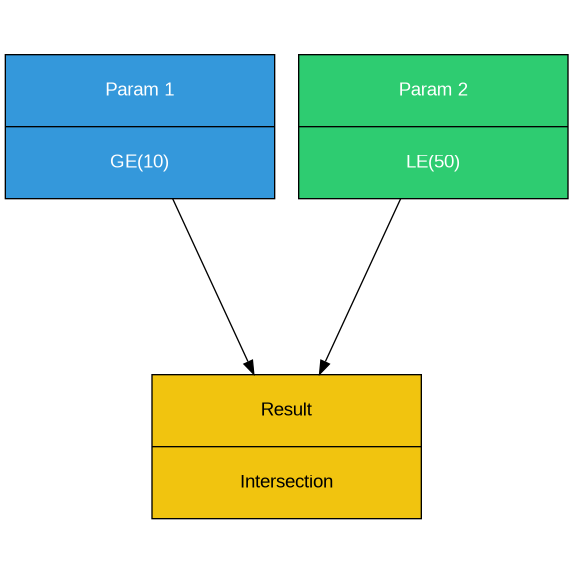
\includegraphics[width=0.9\textwidth]{logic_prog.png}
        \end{column}
        \begin{column}{0.5\textwidth}
            \textbf{How Range Queries Work}:
            \begin{itemize}
                \item \textbf{Trapdoors}: App generates 2 secure search tokens.
                \item \textbf{Server Side}: Returns encrypted match sets.
                \item \textbf{Intersection}: \texttt{BitSequence} logic on phone finds the final result.
            \end{itemize}
        \end{column}
    \end{columns}
\end{frame}

\begin{frame}{Universal Android Support}
    \begin{columns}
        \begin{column}{0.6\textwidth}
            \textbf{Multi-Core Stability}:
            \begin{itemize}
                \item Supports \textbf{arm64-v8a}, \textbf{v7a}, \textbf{x86}, and \textbf{x64}.
                \item High-speed static C++ libraries linked via CMake.
                \item Hardened JNI to prevent native crashes.
            \end{itemize}
        \end{column}
        \begin{column}{0.4\textwidth}
            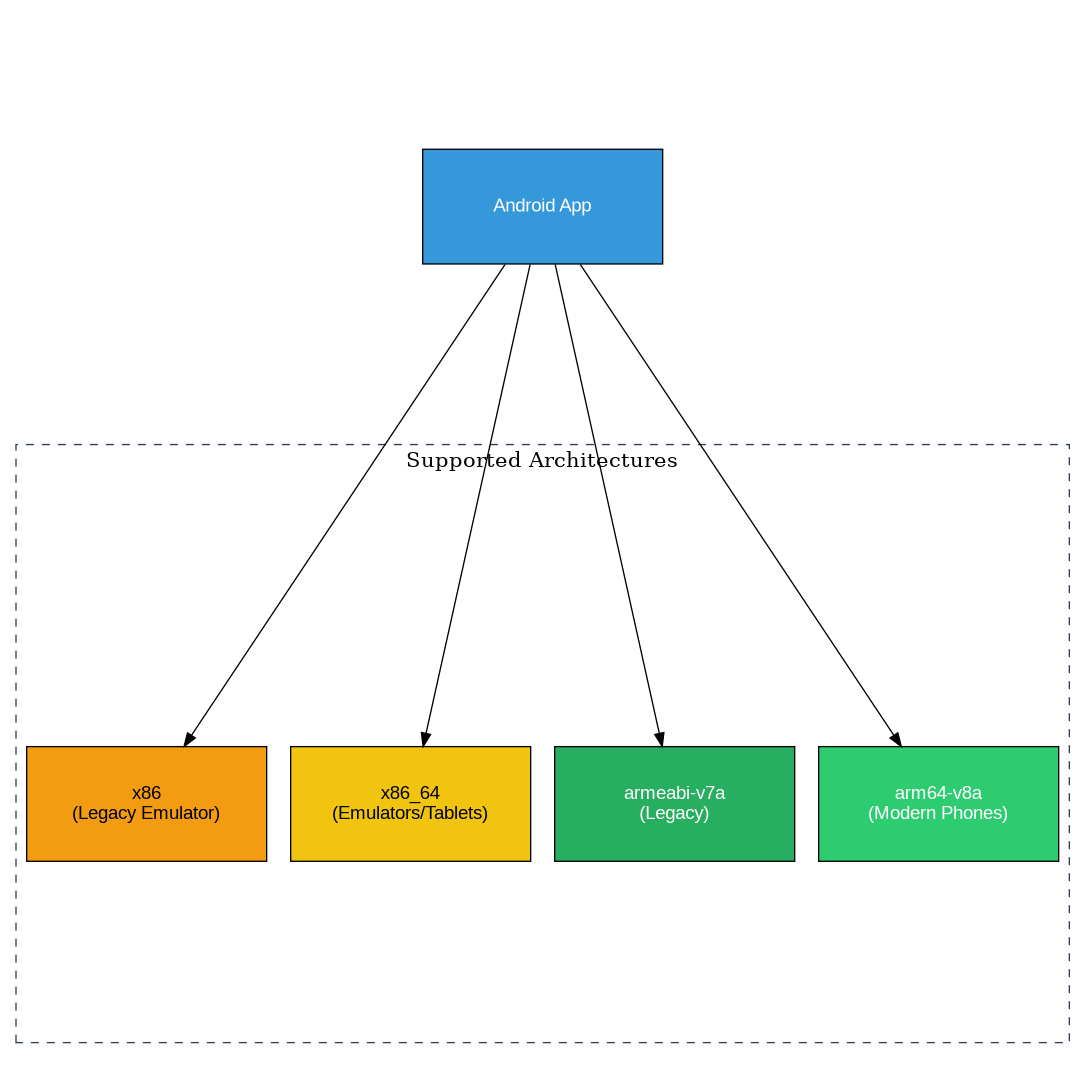
\includegraphics[width=\textwidth]{archs_prog.png}
        \end{column}
    \end{columns}
\end{frame}

\begin{frame}{Server Architecture: Node.js Middleware}
    \begin{columns}
        \begin{column}{0.65\textwidth}
            \begin{itemize}
                \item \textbf{Role}: Acts as a secure REST middleware bridging the Android client with the C++ DSSE Core and File Storage.
                \item \textbf{Decoupling}: Abstracts away complex command-line native executions (RocksDB) into predictable, standard REST calls.
                \item \textbf{Native Integration}: Spawns \texttt{dsse\_server} child processes, feeding large batch updates via \texttt{stdin} streams to bypass OS command-line limits.
            \end{itemize}
        \end{column}
        \begin{column}{0.35\textwidth}
            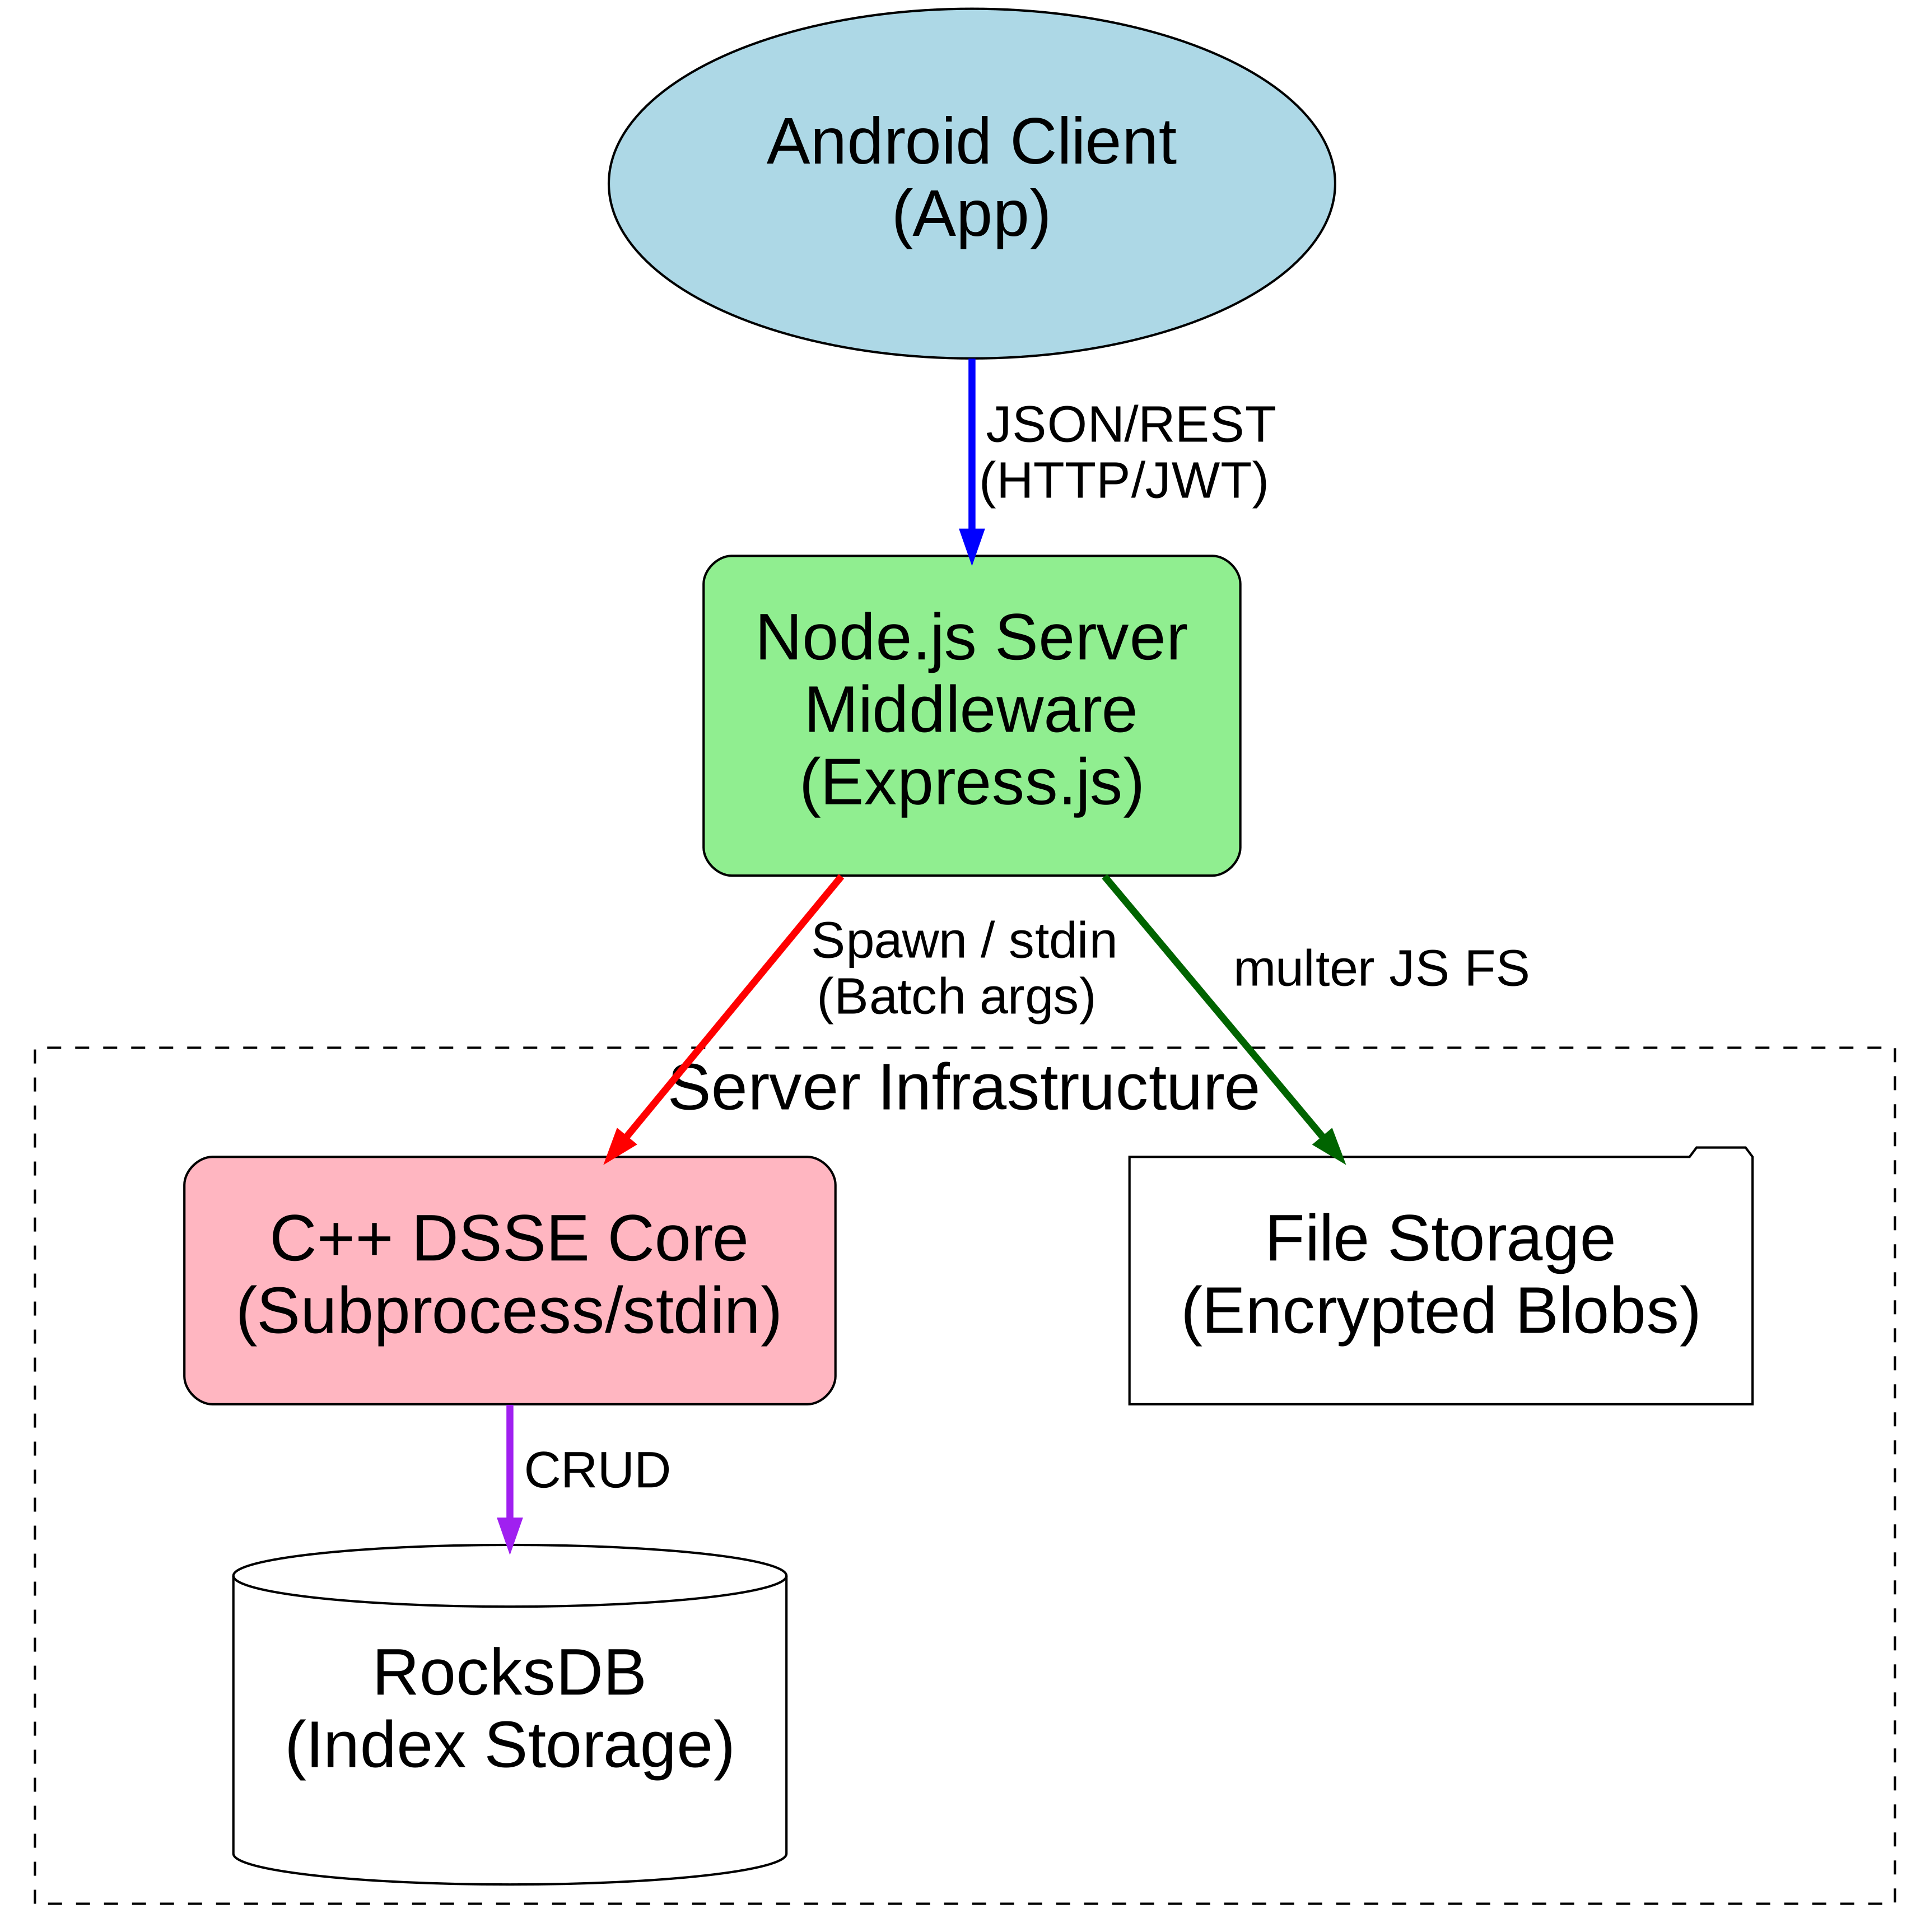
\includegraphics[width=\textwidth]{server_arch.png}
        \end{column}
    \end{columns}
\end{frame}

\begin{frame}{API Endpoints \& Security}
    \begin{columns}
        \begin{column}{0.55\textwidth}
            \textbf{Endpoint Structure \& Purpose}:
            \begin{itemize}
                \item \textbf{Auth} (\texttt{/login}): JWT-based sessions in MongoDB.
                \item \textbf{Space} (\texttt{/new}): Provisions isolated \texttt{DBSpace}.
                \item \textbf{Index} (\texttt{/bulk-save}): Interacts with RocksDB for search/update.
                \item \textbf{File} (\texttt{/upload}): Handles encrypted document blobs.
            \end{itemize}
        \end{column}
        \begin{column}{0.45\textwidth}
            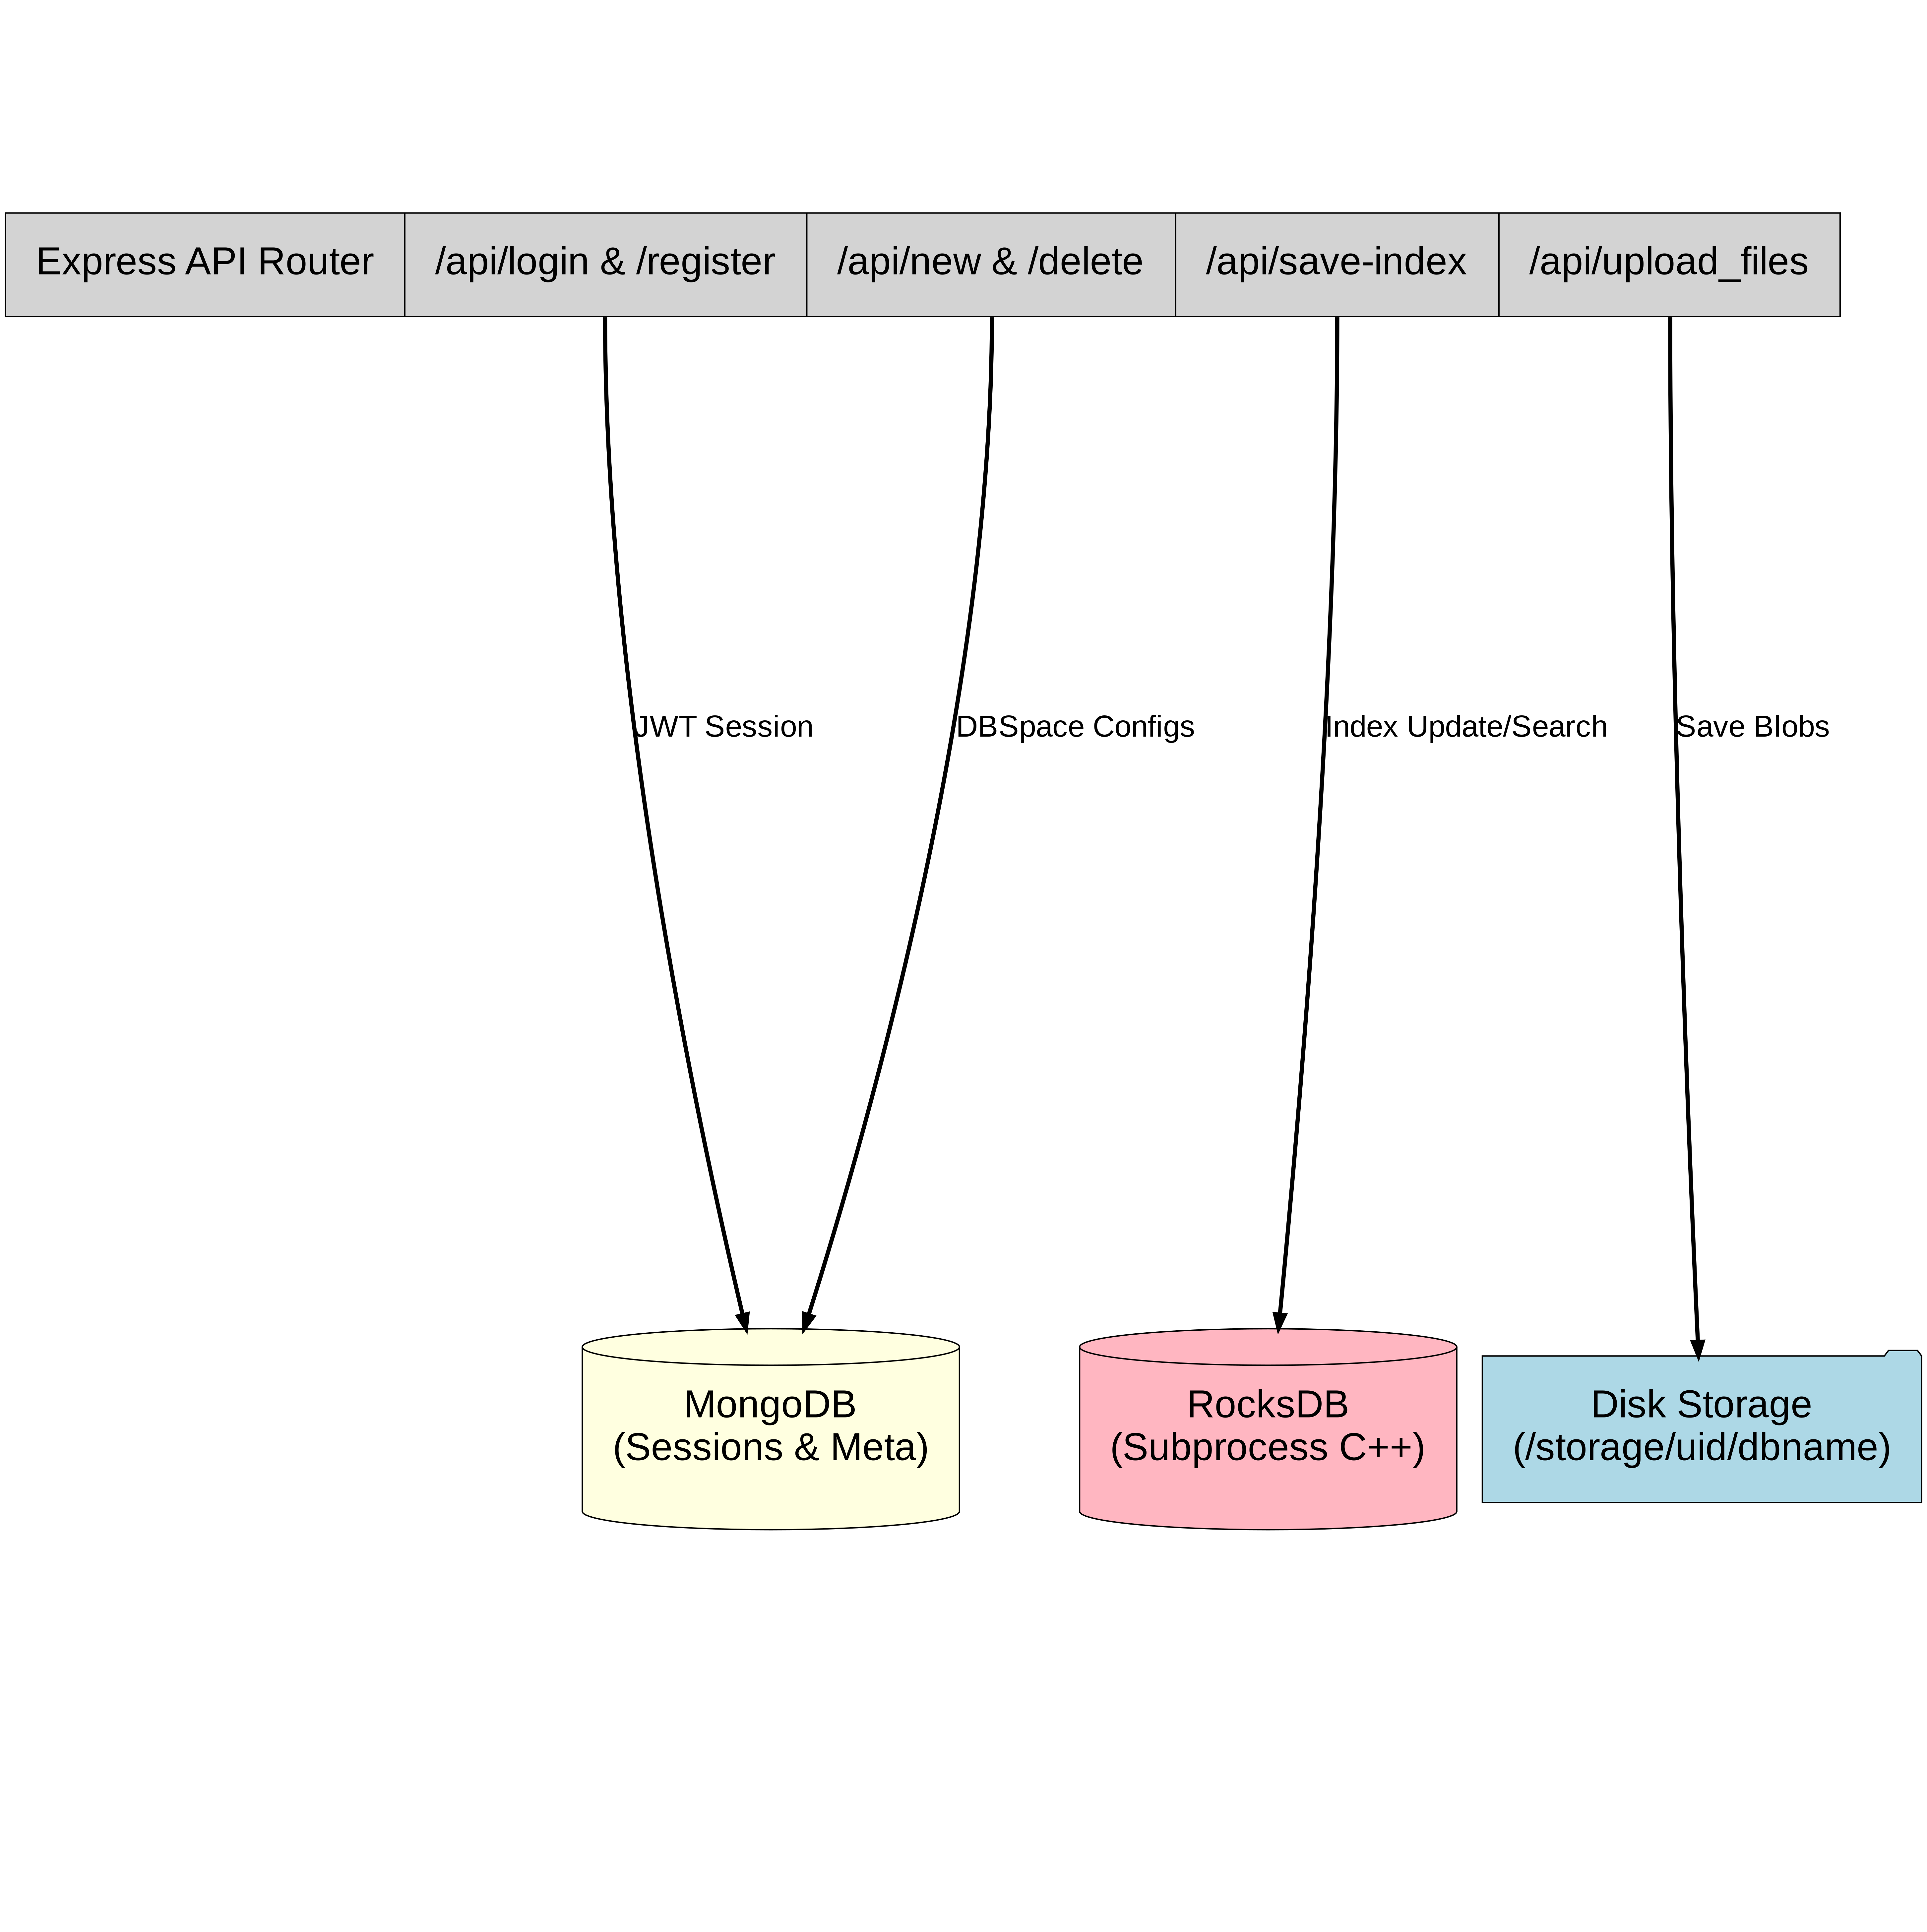
\includegraphics[width=\textwidth]{server_api.png}
        \end{column}
    \end{columns}
\end{frame}

\begin{frame}{Security \& Edge Case Handling}
    \begin{columns}
        \begin{column}{0.65\textwidth}
            \begin{itemize}
                \item \textbf{Zero-Trust}: \texttt{protect} middleware validates JWT AND ownership.
                \item \textbf{Immutable Locks}: Upon completion, the App triggers \texttt{/lock-space}. The API irrevocably sets \texttt{isLocked=true} in Mongo, physically preventing hackers from re-uploading and destroying the RocksDB index.
                \item \textbf{Anti-Path Traversal}: Verifies \texttt{startsWith()} against \texttt{../} attacks.
                \item \textbf{Dynamic Storage}: \texttt{multer} safely resolves path before bytes read.
            \end{itemize}
        \end{column}
        \begin{column}{0.35\textwidth}
            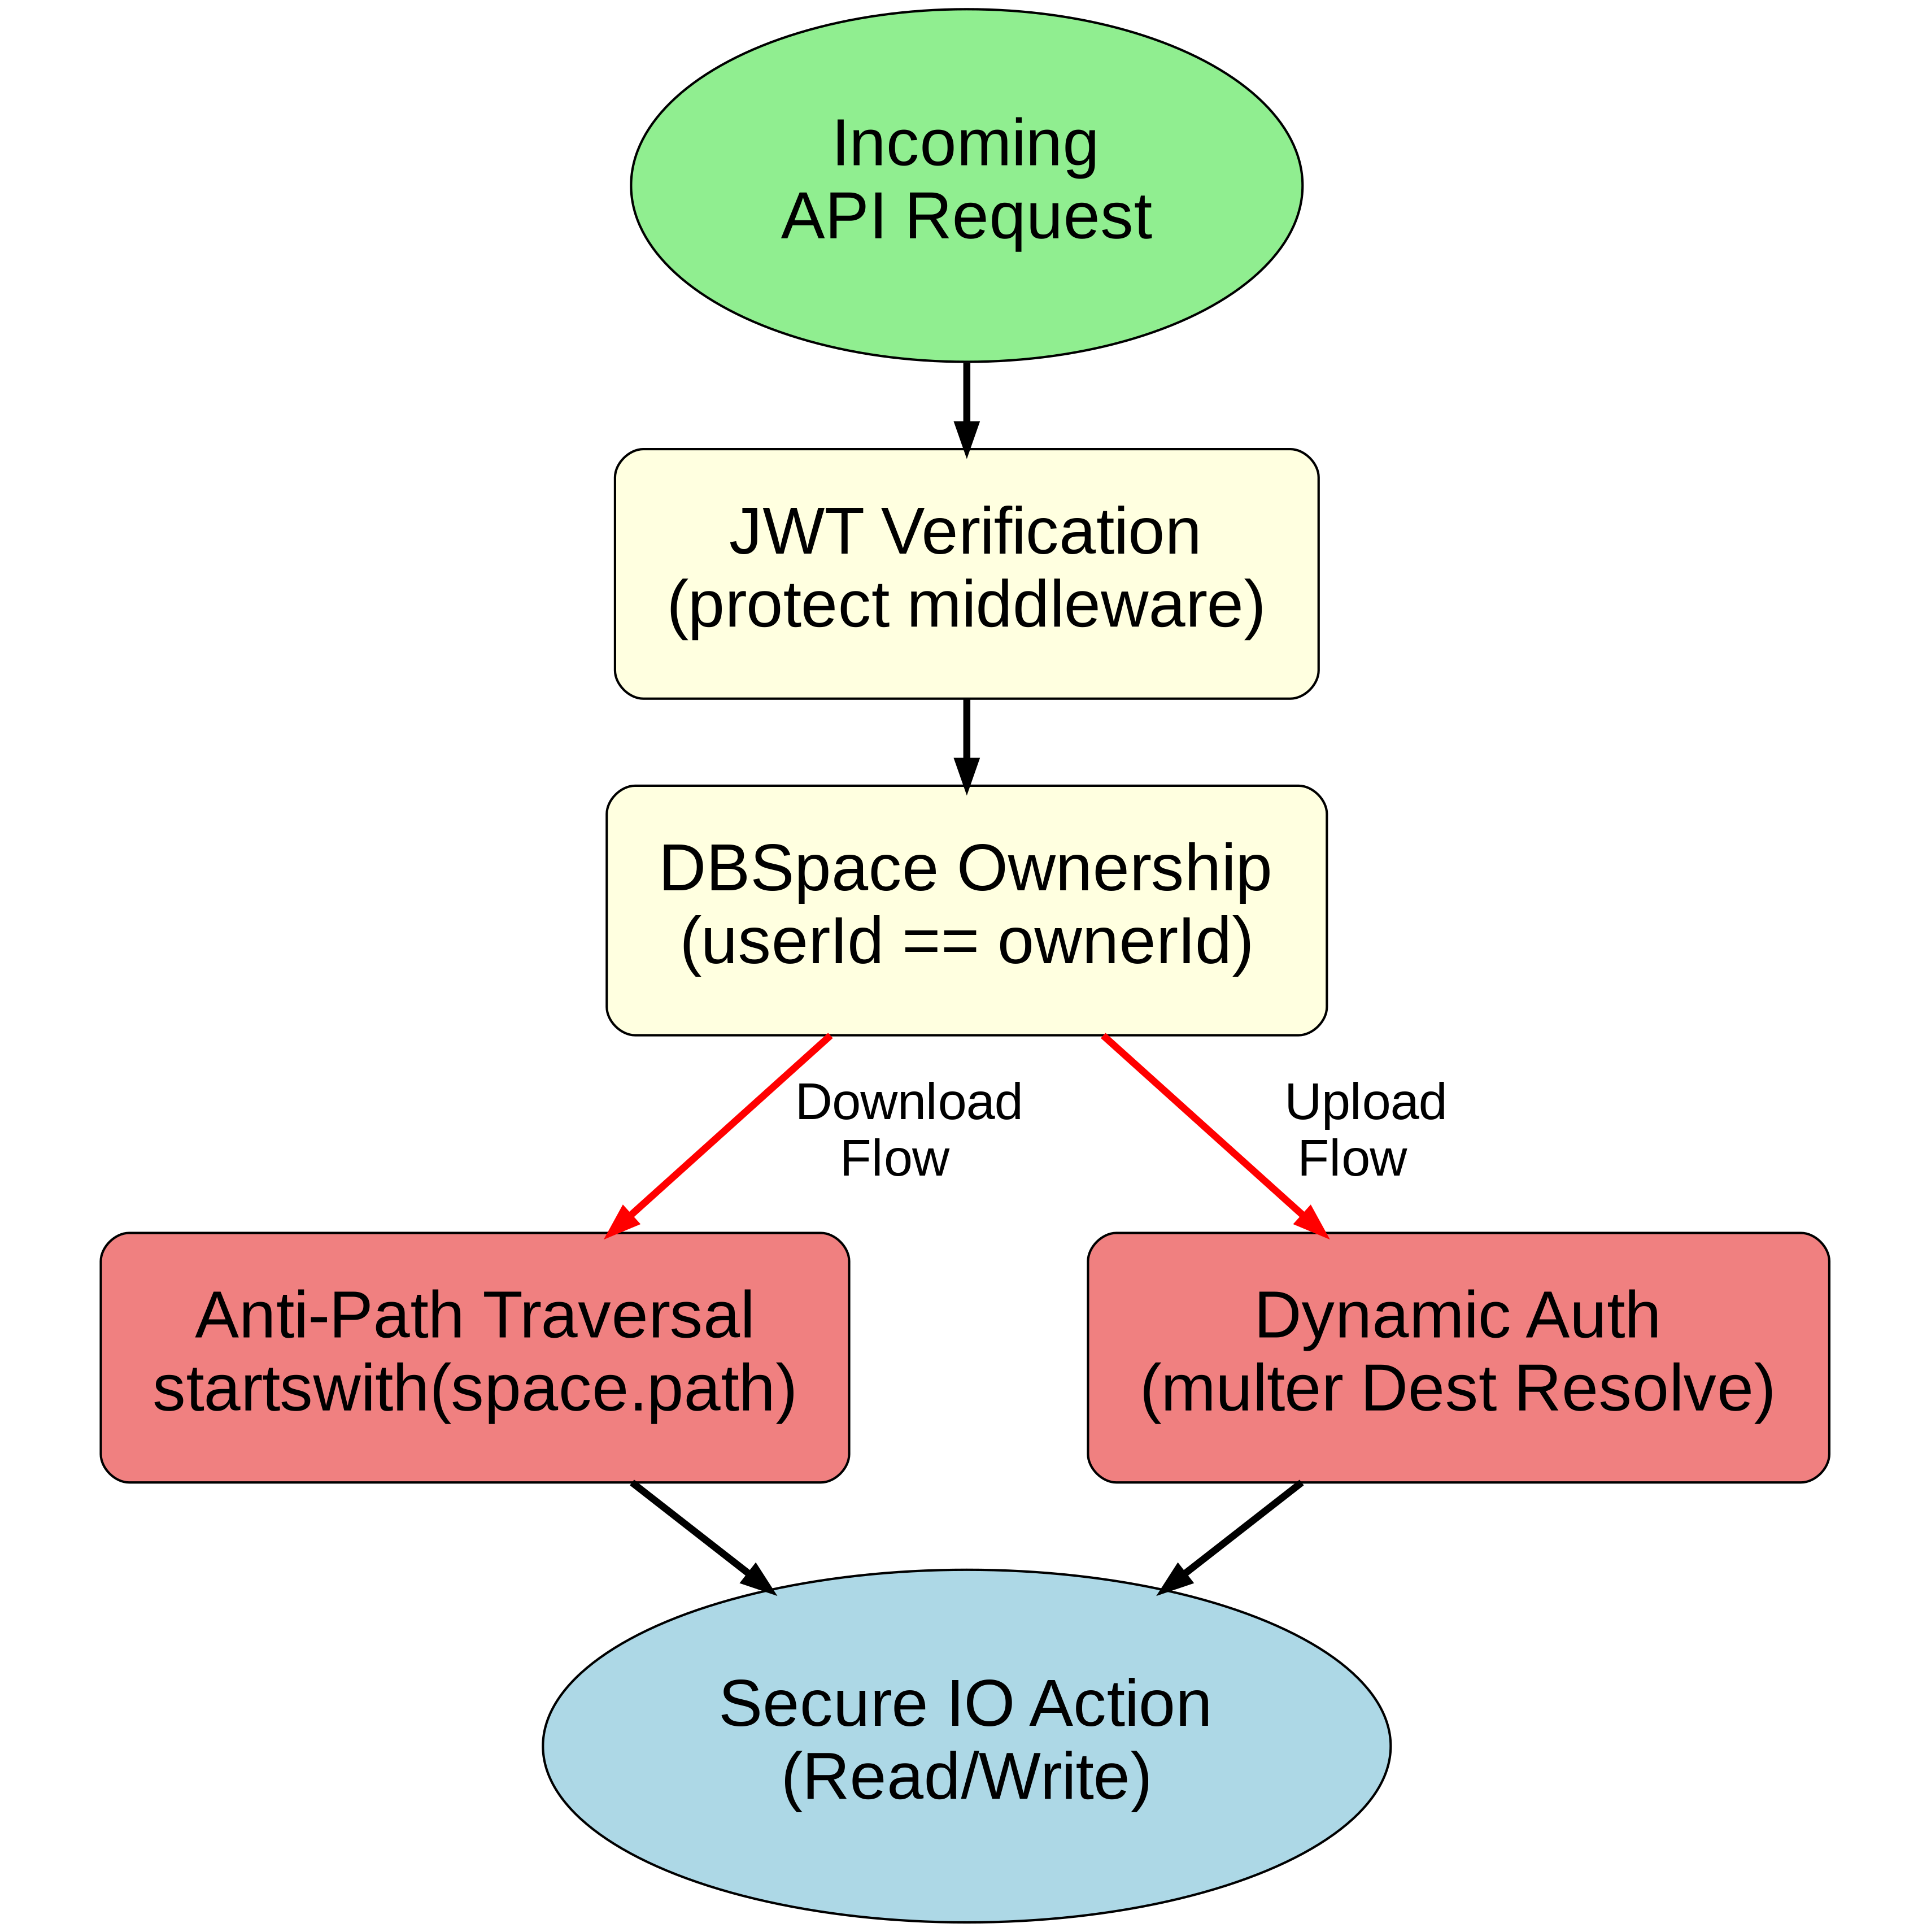
\includegraphics[width=\textwidth]{server_sec.png}
        \end{column}
    \end{columns}
\end{frame}

\begin{frame}{Cryptographic Core: The FAST Scheme}
    \begin{columns}
        \begin{column}{0.65\textwidth}
            \begin{itemize}
                \item \textbf{C++ \& NDK}: High performance native cryptographic routines using \texttt{Crypto++}.
                \item \textbf{Master Key Derivation}: Initial AES-256 keys generate subsequent sub-keys via Pseudo-Random Number Generators (PRNG).
                \item \textbf{HMAC-SHA256}: Encrypts both the file paths and search keywords into Trapdoor Tokens.
                \item \textbf{Local Counters}: Phone retains state integers via a local RocksDB preventing duplicate tokens.
            \end{itemize}
        \end{column}
        \begin{column}{0.35\textwidth}
            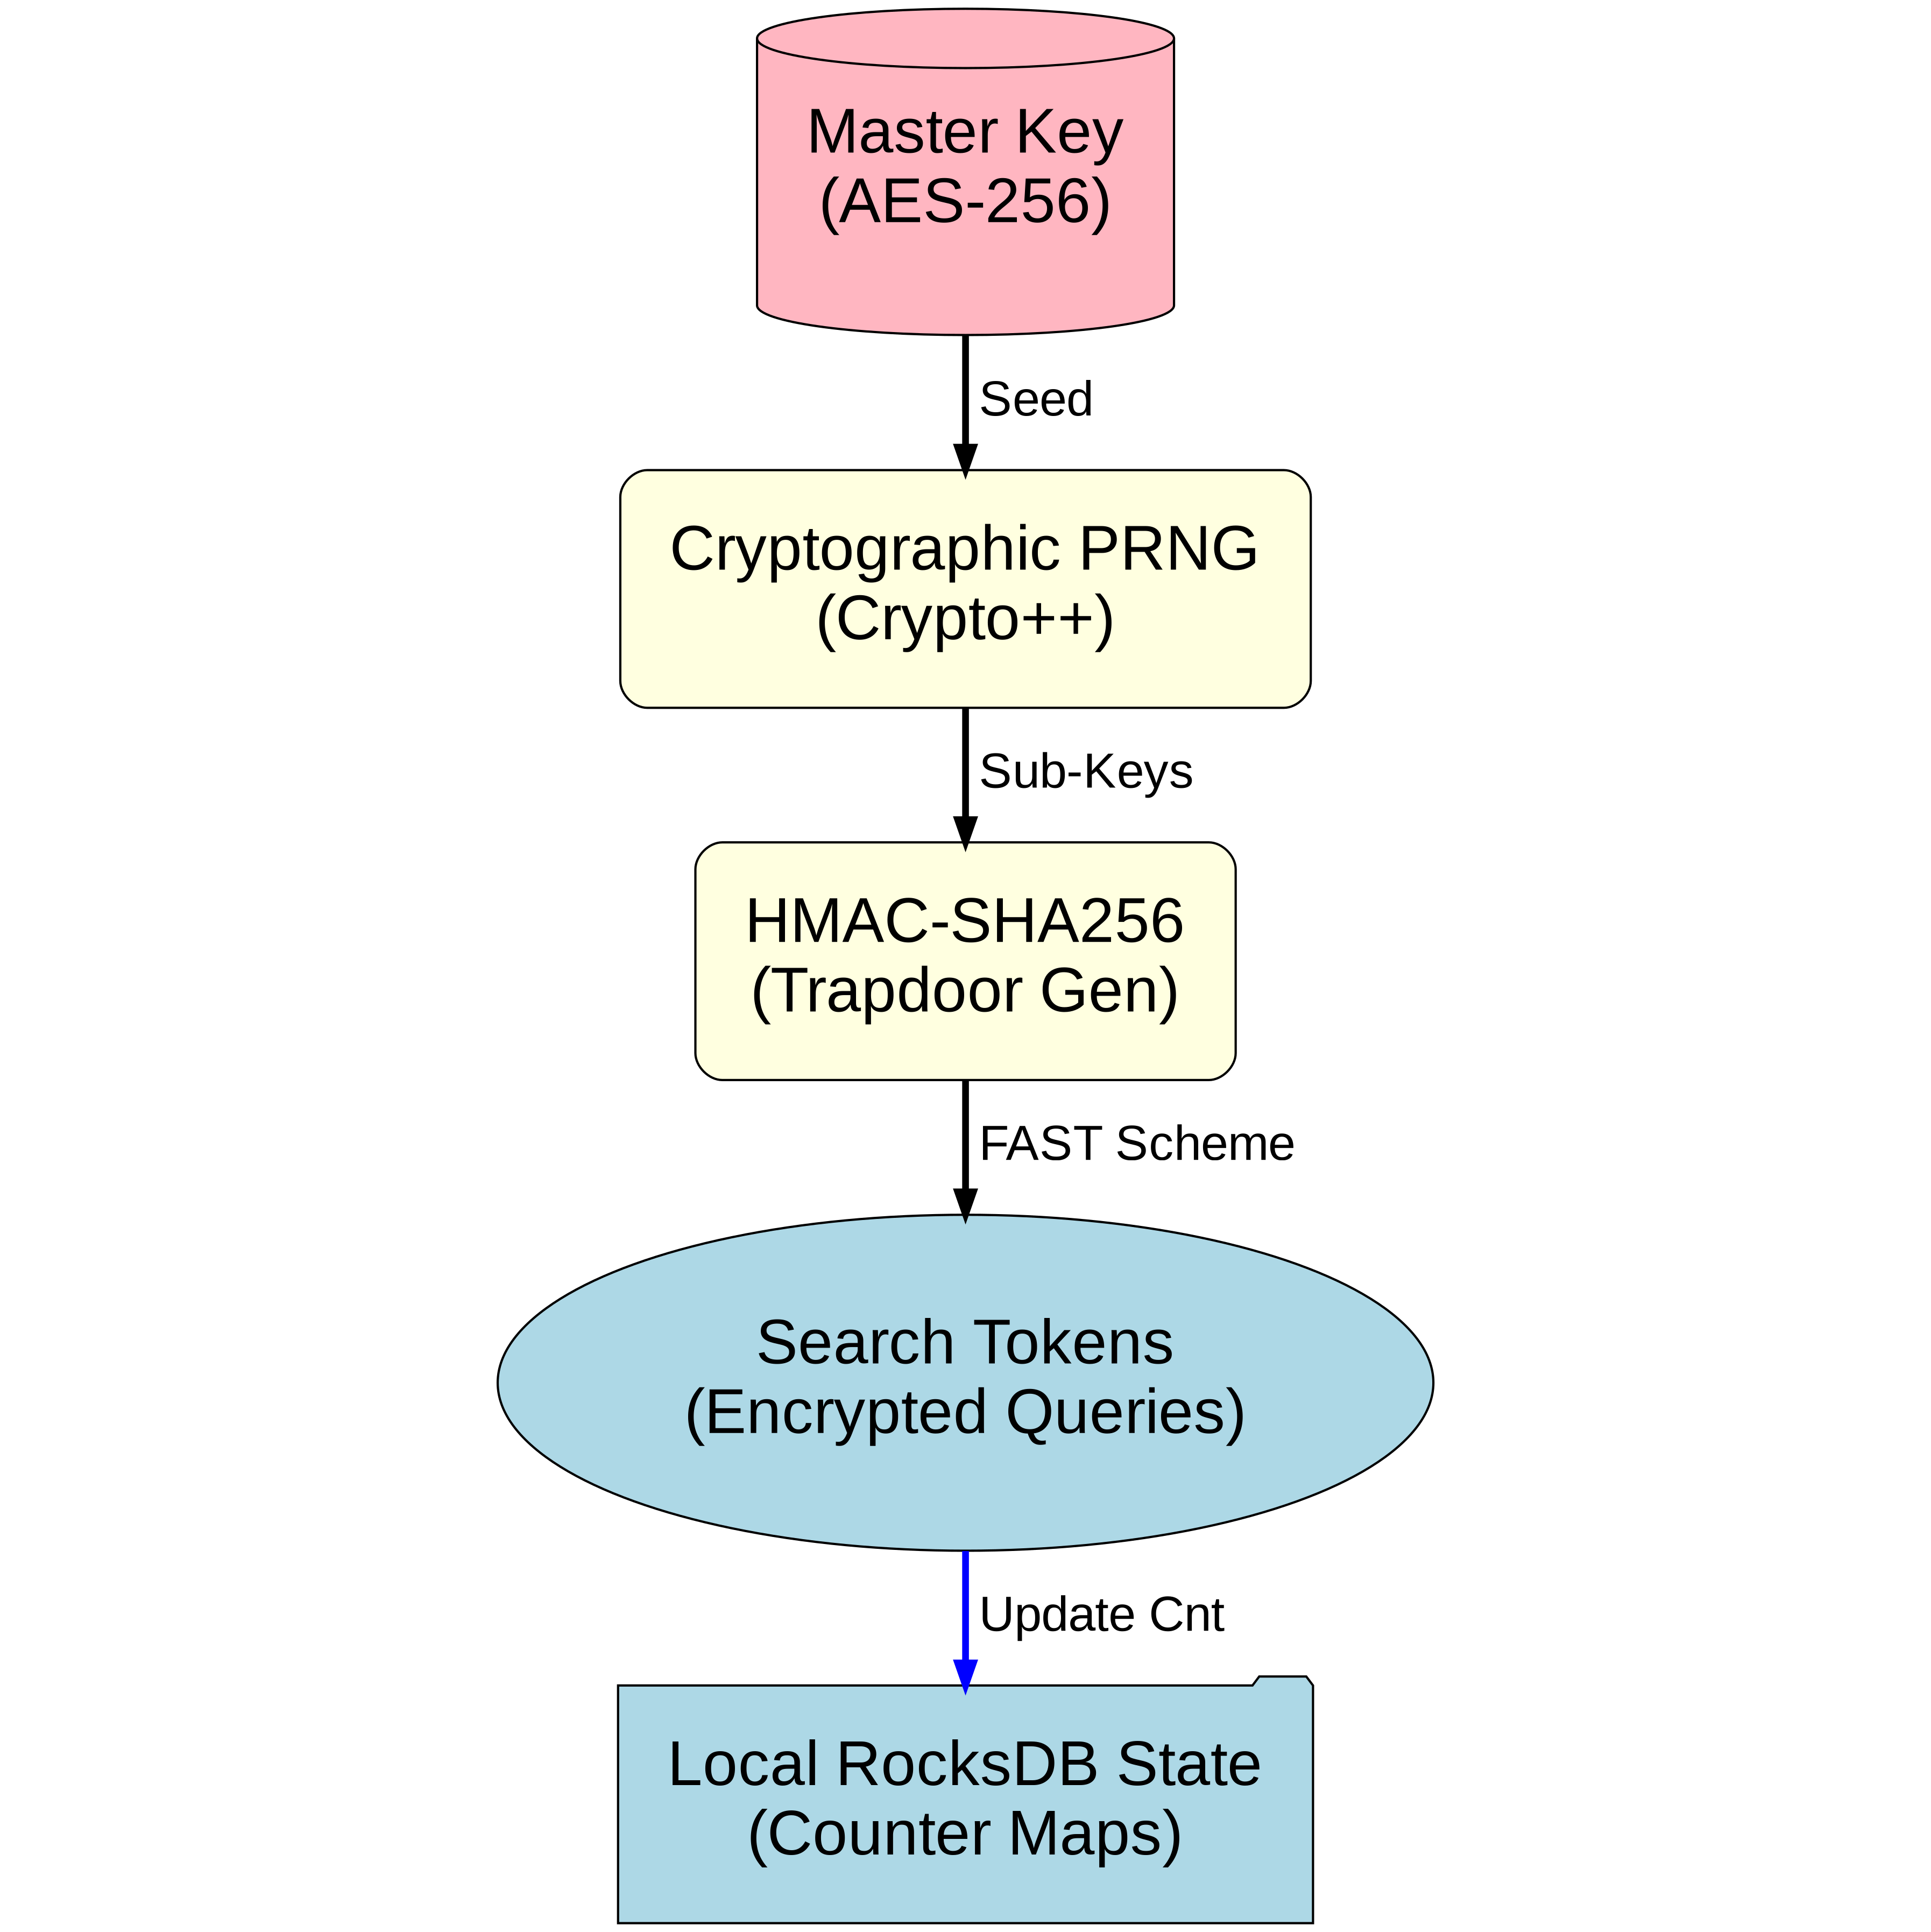
\includegraphics[width=\textwidth]{crypto_core.png}
        \end{column}
    \end{columns}
\end{frame}

\begin{frame}{Multi-Tenant Storage Isolation}
    \begin{columns}
        \begin{column}{0.65\textwidth}
            \begin{itemize}
                \item \textbf{Complete Compartmentalization}: Each user's database is a 100\% physically separate folder on the Linux server filesystem.
                \item \textbf{JWT $\rightarrow$ UID Mapping}: The API extracts the authenticated UID from the Bearer Token, never trusting the client's payload.
                \item \textbf{MongoDB Lookup}: The DBSpace schema strictly links the requested database name to the verified UID to extract the true absolute path (\texttt{/storage/uid\_XYZ/dbname/}).
            \end{itemize}
        \end{column}
        \begin{column}{0.35\textwidth}
            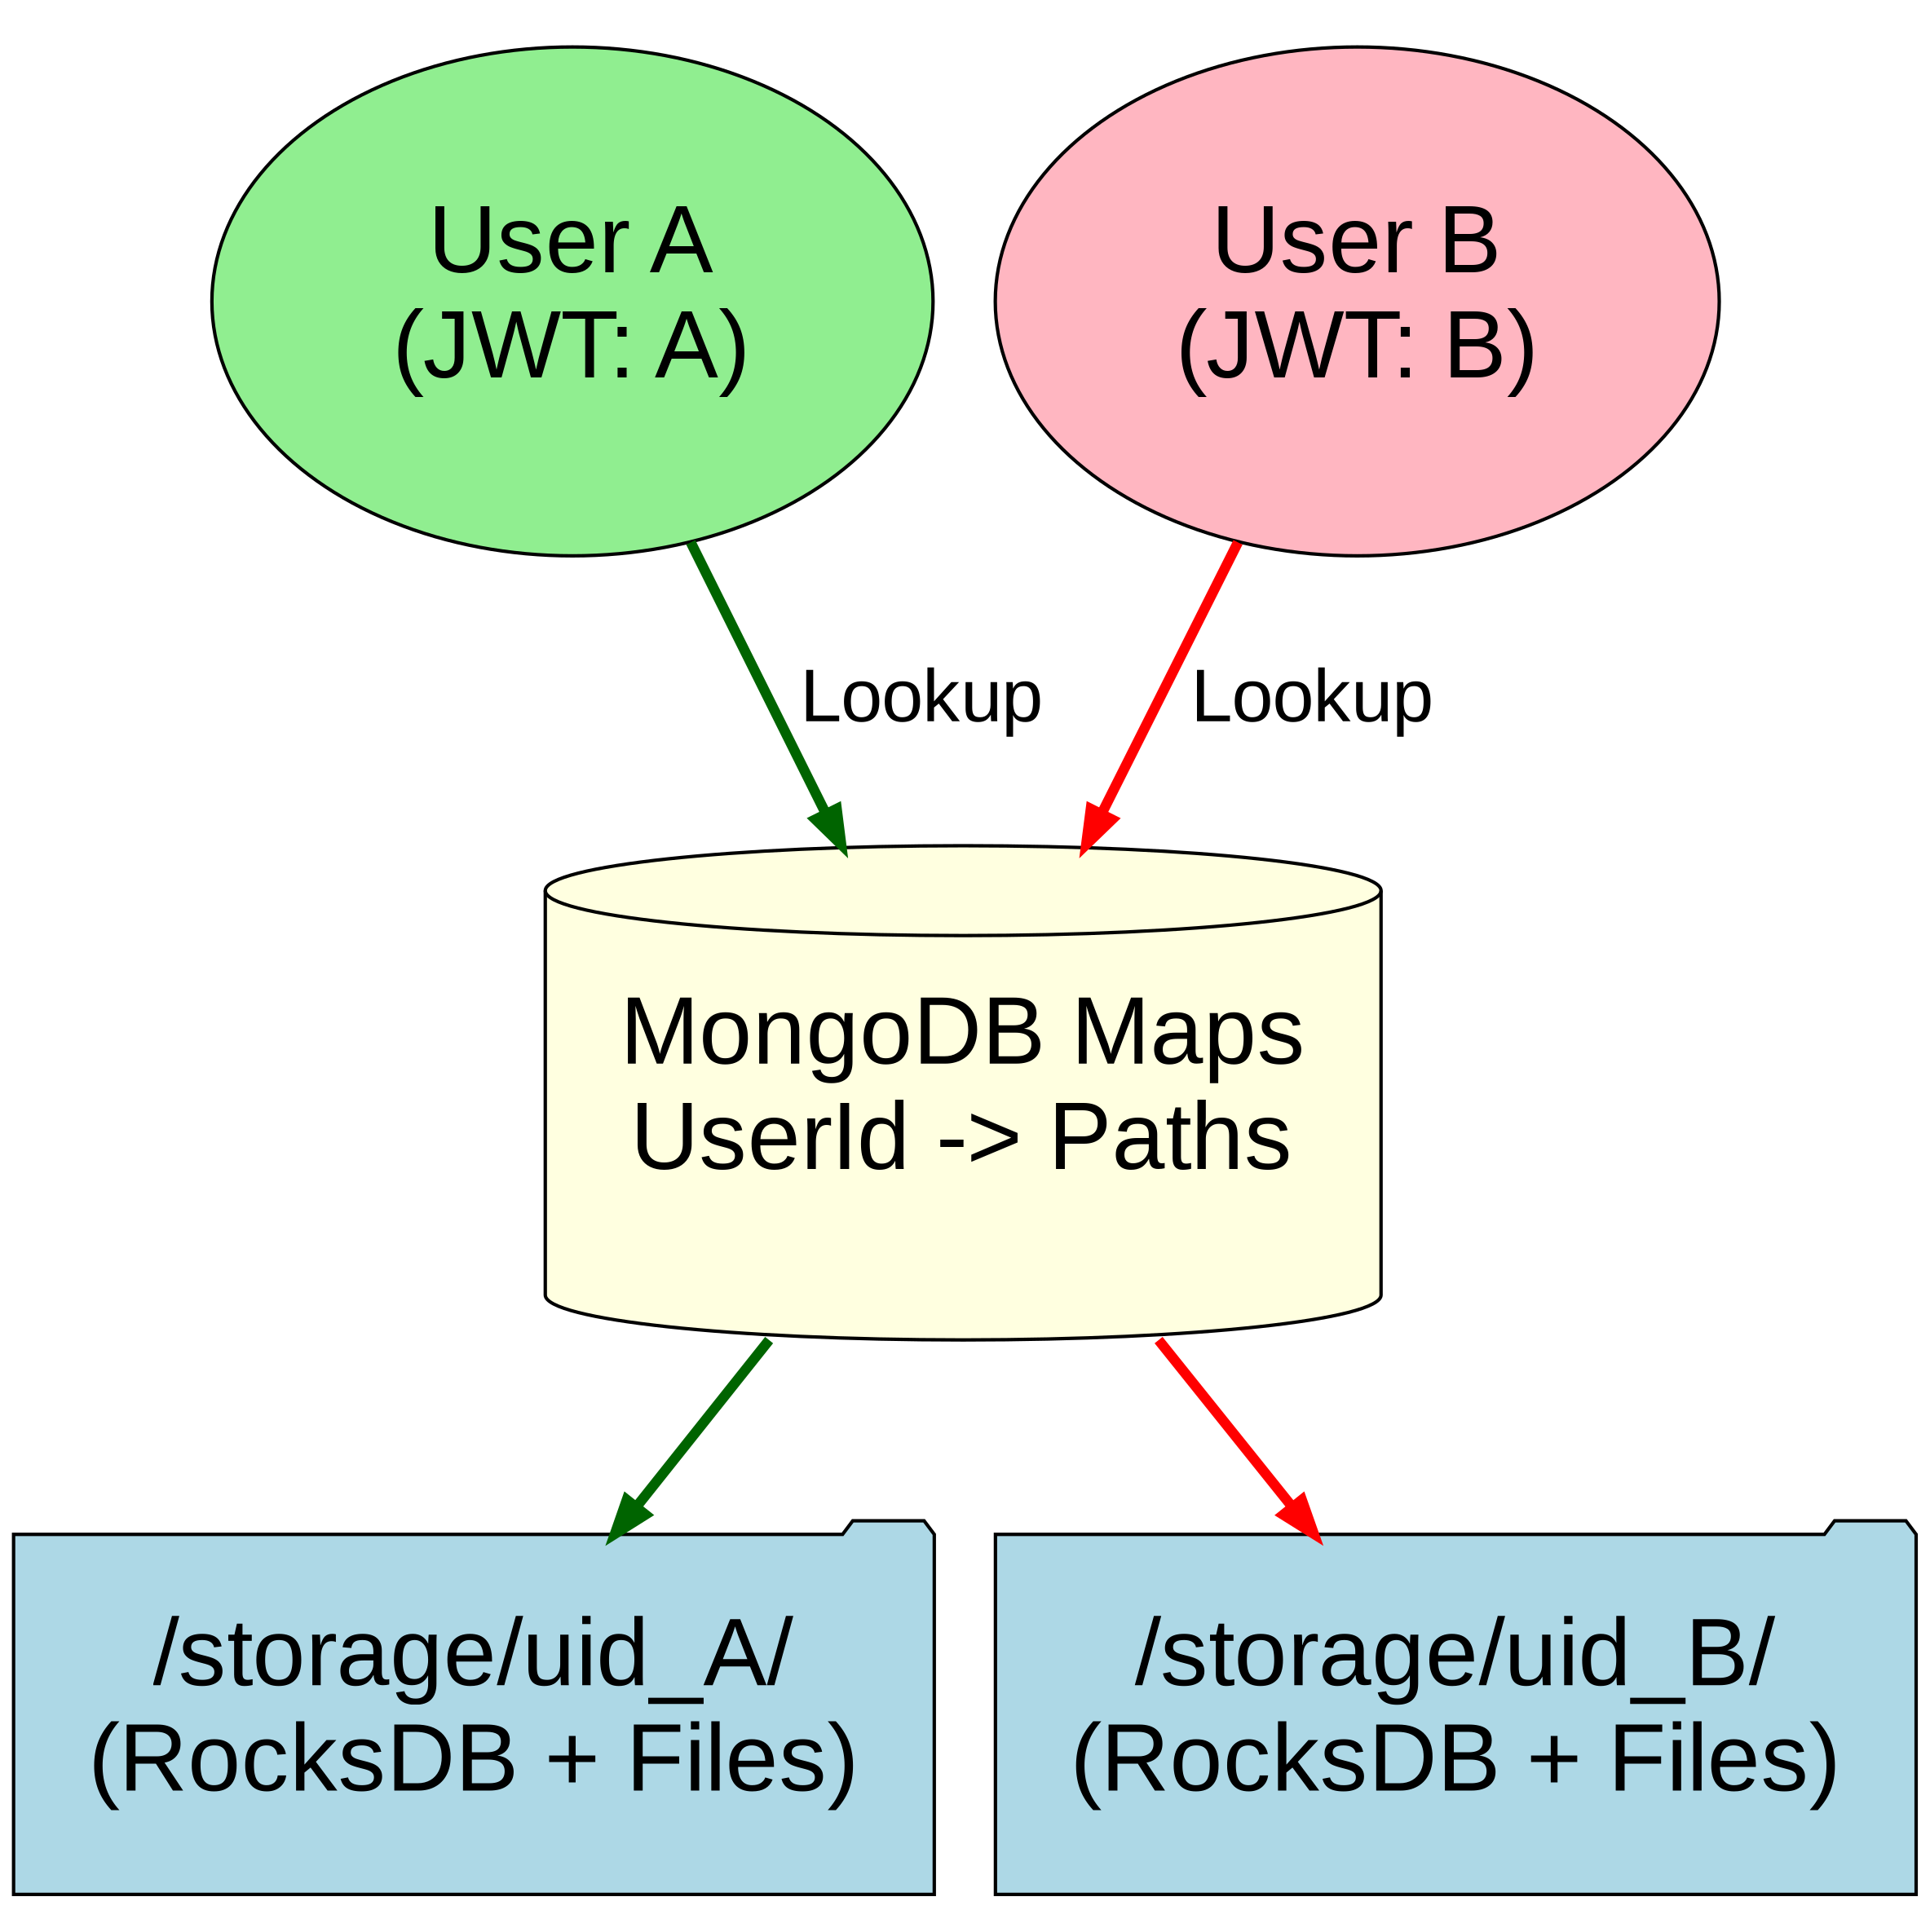
\includegraphics[width=\textwidth]{tenant_isolation.png}
        \end{column}
    \end{columns}
\end{frame}

\begin{frame}{Granular Download Control: Logic Flow}
    \centering
    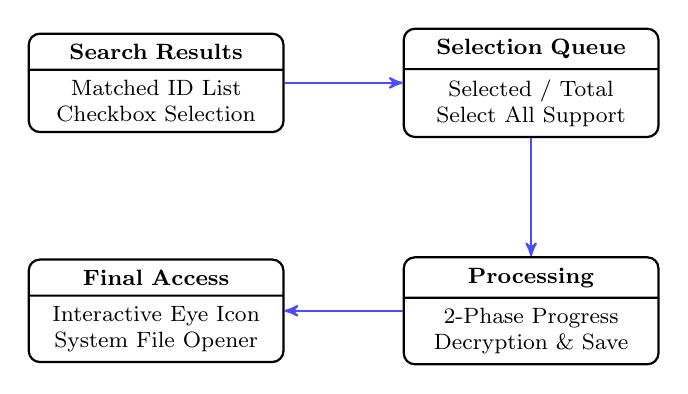
\begin{tikzpicture}[auto, >=stealth', thick,
        block/.style={rectangle split, rectangle split parts=2, draw, rounded corners, text width=3cm, align=center, font=\footnotesize},
        header/.style={fill=blue!70, text=white, font=\footnotesize\bfseries},
        content/.style={fill=blue!10}]

        \node [block] (search) {
            \nodepart{one} \textbf{Search Results}
            \nodepart{two} Matched ID List \\ Checkbox Selection
        };

        \node [block, right=of search, xshift=0.5cm] (queue) {
            \nodepart{one} \textbf{Selection Queue}
            \nodepart{two} Selected / Total \\ Select All Support
        };

        \node [block, below=of queue, yshift=-0.5cm] (stream) {
            \nodepart{one} \textbf{Processing}
            \nodepart{two} 2-Phase Progress \\ Decryption \& Save
        };

        \node [block, left=of stream, xshift=-0.5cm] (view) {
            \nodepart{one} \textbf{Final Access}
            \nodepart{two} Interactive Eye Icon \\ System File Opener
        };

        \draw[->, thick, blue!70] (search) -- (queue);
        \draw[->, thick, blue!70] (queue) -- (stream);
        \draw[->, thick, blue!70] (stream) -- (view);
    \end{tikzpicture}
    \vspace{0.4cm}
    \begin{itemize}
        \item \textbf{Efficiency}: Targeted downloads reduce server load.
        \item \textbf{UX}: Instant visual feedback with green success states.
    \end{itemize}
\end{frame}

\begin{frame}{UX Architecture: Live Monitoring}
    \begin{itemize}
        \item \textbf{Luxury Visuals}: Midnight Surface with Luxury Gold branding.
        \item \textbf{2-Phase Interactive Progress}:
            \begin{itemize}
                \item \textbf{Phase 1 (Gold)}: Real-time network stream tracking (0--80\%).
                \item \textbf{Phase 2 (Green)}: Post-decryption success verification (100\%).
            \end{itemize}
        \item \textbf{Adaptability}: Full \texttt{fitsSystemWindows} support for hardware bezels.
        \item \textbf{Stable Scrolling}: Nested scroll containers prevent layout shifting with dense data.
    \end{itemize}
\end{frame}

\begin{frame}{App Functionality Summary}
    \begin{enumerate}
        \item \textbf{Login}: Secure JWT session establishment.
        \item \textbf{Update}: Batch token generation \& file encryption.
        \item \textbf{Search}: Range query with \textbf{Manual Selection Control}.
        \item \textbf{Live Recovery}: 2-phase tracking with \textbf{Integrated Viewing}.
    \end{enumerate}
\end{frame}

\begin{frame}{DEMO: The Storage Challenge}
    \begin{columns}
        \begin{column}{0.45\textwidth}
            \textbf{Problem Statement}:
            \begin{itemize}
                \item \textbf{Data}: Tax Defaulter PDFs
                \item \textbf{Issue}: Phone storage full
                \item \textbf{Risk}: Untrusted Cloud
            \end{itemize}
        \end{column}
        \begin{column}{0.55\textwidth}
            \centering
            \resizebox{\textwidth}{!}{
            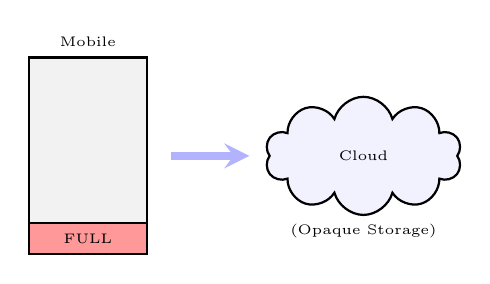
\begin{tikzpicture}[>=stealth, thick]
                % Phone
                \draw[fill=gray!10] (0,0) rectangle (1.5,2.5);
                \draw[fill=red!40] (0,0) rectangle (1.5,0.4) node[midway, font=\tiny] {FULL};
                \node at (0.75, 2.7) {\tiny Mobile};
                
                % Arrow
                \draw[->, line width=1mm, blue!30] (1.8,1.25) -- (2.8,1.25);
                
                % Cloud
                \node[cloud, draw, fill=blue!5, minimum width=2.5cm, minimum height=1.5cm] at (4.25,1.25) {\tiny Cloud};
                \node at (4.25, 0.3) {\tiny (Opaque Storage)};
            \end{tikzpicture}
            }
        \end{column}
    \end{columns}
\end{frame}

\begin{frame}{DEMO: The PI Searchable Workflow}
    \centering
    \resizebox{0.9\textwidth}{!}{
    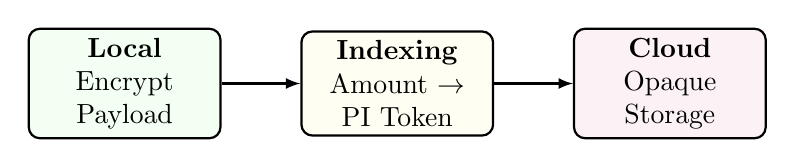
\begin{tikzpicture}[node distance=1cm, auto, >=latex, thick]
        \node [draw, fill=green!5, rounded corners, text width=2.2cm, align=center] (local) {\textbf{Local}\\Encrypt Payload};
        \node [draw, fill=yellow!5, rounded corners, right=of local, text width=2.2cm, align=center] (index) {\textbf{Indexing}\\Amount $\rightarrow$ PI Token};
        \node [draw, fill=purple!5, rounded corners, right=of index, text width=2.2cm, align=center] (cloud) {\textbf{Cloud}\\Opaque Storage};
        
        \draw[->] (local) -- (index);
        \draw[->] (index) -- (cloud);
    \end{tikzpicture}
    }
    \vspace{0.8cm}
    \begin{itemize}
        \item \textbf{Zero Visibility}: Server only stores bit-pattern indexes.
        \item \textbf{Selective Control}: Phone requests only what it needs.
    \end{itemize}
\end{frame}

\begin{frame}{DEMO: Tax Defaulter Dataset Sample}
    \centering
    \resizebox{0.8\textwidth}{!}{
    \begin{tabular}{|l|l|l|}
        \hline
        \rowcolor{blue!10} \textbf{File (Keyword)} & \textbf{Taxpayer Name} & \textbf{Status} \\ \hline
        99286.pdf & Sofia Oliveira & \textcolor{red}{Defaulter} \\
        74127.pdf & Li Wei & \textcolor{red}{Defaulter} \\
        65386.pdf & Lucas Muller & \textcolor{red}{Defaulter} \\
        58625.pdf & John Smith & \textcolor{red}{Defaulter} \\
        14747.pdf & Maria Garcia & \textcolor{red}{Defaulter} \\ \hline
    \end{tabular}
    }
    \par\vspace{0.5cm}
    \small{\textit{Amounts (14k--99k) serve as secure range-search keywords.}}
\end{frame}

\begin{frame}{DEMO: Range Query [\$50k -- \$75k]}
    \begin{columns}
        \begin{column}{0.5\textwidth}
            \textbf{In-App Query}:
            \begin{itemize}
                \item \textbf{Input}: Range [50k, 75k]
                \item \textbf{Trapdoor}: Client secret
                \item \textbf{Retrieve}: 3 Files
            \end{itemize}
        \end{column}
        \begin{column}{0.5\textwidth}
            \centering
            \resizebox{\textwidth}{!}{
            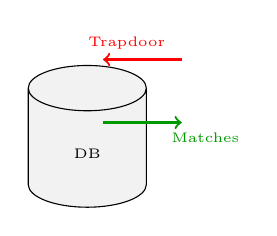
\begin{tikzpicture}
                \node[draw, cylinder, fill=gray!10, shape border rotate=90, minimum width=1.5cm, minimum height=1.8cm] (db) {\tiny DB};
                \draw[->, red, thick] (1.2,1.2) -- (0.2,1.2) node[above, xshift=0.3cm, font=\tiny] {Trapdoor};
                \draw[->, green!60!black, thick] (0.2,0.4) -- (1.2,0.4) node[below, xshift=0.3cm, font=\tiny] {Matches};
            \end{tikzpicture}
            }
        \end{column}
    \end{columns}
    \vspace{1cm}
    \begin{center}
        \fcolorbox{green}{white}{\textbf{Outcome}: Only relevant files retrieved via Range Query.}
    \end{center}
\end{frame}

\end{document}
